\subsection{Structures}

\subsection{Unit Construction Structures}

-talk about a generic unit building structure

-building mode has seperate actions for each type of troop with an assigned probability

-update this image using the existing scv powerpoint as a template

\begin{figure}
\centering
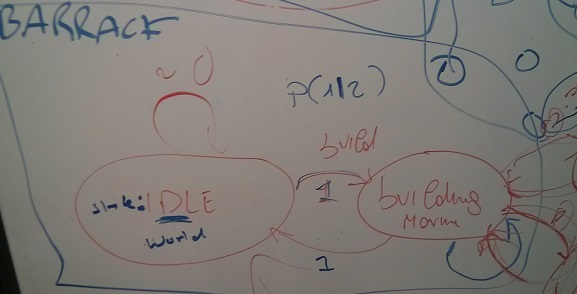
\includegraphics[scale=0.8, trim = 0cm 0cm 0cm 0cm]{diagrams/barracks}
\label{fig:barracks_diagram}
\caption{Markov Chain for unit building structures.}
\end{figure}

\subsection{Research Orientated Structures}

-create a similar generic diagram for research structures

-indicate using states how certain options are cut off